Extracting structured information from unstructured text has been a central challenge in natural language processing (NLP) for decades. Early systems were rule-based, using handcrafted grammars, dictionaries, and regular expressions to detect domain-specific patterns \cite{grishman1997information}. These methods worked well in narrow settings but were brittle, required heavy manual effort, and could not easily adapt to new domains.

Statistical models offered more flexibility. Hidden Markov Models (HMMs) were used to model sequential dependencies, while Conditional Random Fields (CRFs) became particularly influential by enabling richer feature-based sequence labeling \cite{sarawagi2008information}. CRFs were widely adopted for tasks such as Named Entity Recognition (NER) and slot filling, achieving strong results on shared tasks like CoNLL-2003 \cite{tjong2003introduction}. Despite these advances, statistical models still struggled with domain transfer, long-range dependencies, and their reliance on handcrafted features.

Another important limitation of early work was the reliance on pipeline-based architectures. Classical information extraction was usually divided into subtasks such as entity recognition, relation classification, and template alignment. Each stage depended on the output of the previous one, which often led to error propagation \cite{jurafsky2023speech}. For example, if the entity recognition module mislabeled an organization, that error would carry over to relation classification and template population. While pipelines offered modularity, they lacked robustness and transparency, making them hard to apply in noisy or domain-specific environments.

A major breakthrough came with the transformer architecture \cite{vaswani2017attention}. Transformers introduced self-attention and large-scale pretraining, which made it possible to capture long-range context and resolve ambiguity in ways earlier models could not. Building on this foundation, large language models (LLMs) can now generate structured outputs directly, for example in JSON, XML, or task-specific templates. This has enabled information extraction to be performed in zero-shot or few-shot settings, significantly reducing the need for task-specific labeled data \cite{brown2020language,wei2022emergent}. This marks a shift from extractive, pipeline-based designs to generative, end-to-end systems.

One influential contribution in this direction is the work of Du, Rush, and Cardie on \textit{Template Filling with Generative Transformers} \cite{du2021template}. Their framework replaces the traditional two-step pipeline of NER followed by event classification with a single generative system. The model conditions on document tokens and event type markers to generate slot fillers directly. This design captures dependencies across multiple events in one document, avoiding the error propagation typical of pipelines. On the MUC-4 dataset, their approach outperformed both pipeline-based and extractive neural baselines, especially for documents that described multiple events.

\begin{figure}
    \centering
    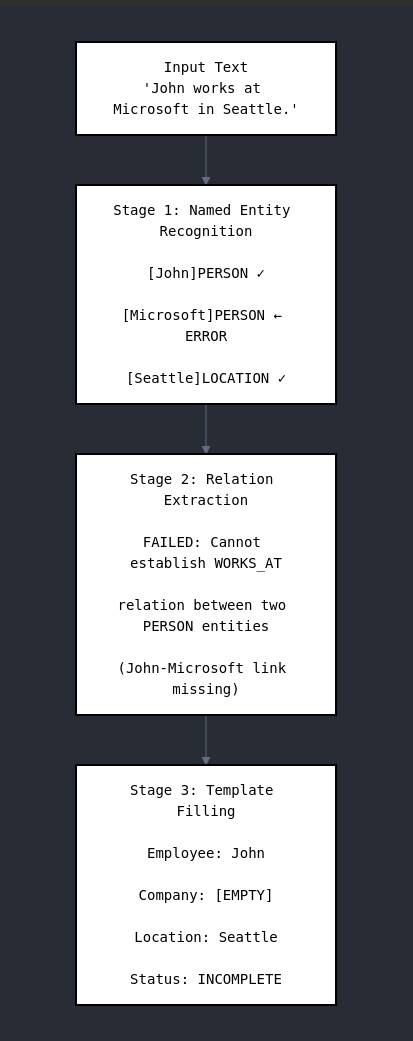
\includegraphics[width=0.6\linewidth]{images/error_propagation.png}
    \caption{Error Propagation Illustration}
    \label{fig:placeholder}
\end{figure}

Benchmarks have played a crucial role in driving research in this area. The MUC-4 dataset \cite{chinchor1992muc} defined an early template filling task for terrorism-related news reports. The ACE program \cite{doddington2004ace} expanded the scope by introducing entity, relation, and event extraction benchmarks across domains. CoNLL-2003 \cite{tjong2003introduction} provided a widely used benchmark for NER in English and German newswire. More recently, speech-based datasets such as SLURP \cite{bastianelli2020slurp} have enabled evaluation of spoken language understanding and slot filling. These benchmarks revealed both the strengths and weaknesses of successive methods, showing where statistical approaches failed and where generative models improved performance. However, they also highlighted the limitations of surface-level metrics such as precision, recall, and F1, which do not capture issues like consistency or robustness.

Despite these advances, domain-specific challenges remain. In healthcare, systems must handle specialized terminology, abbreviations, and implicit knowledge that may not be stated explicitly \cite{friedman2004survey}. In manufacturing and industrial contexts, extraction is complicated by technical identifiers, inconsistent documentation, and informal reporting styles often found in shift logs or maintenance notes \cite{wang2021slu}. These domains require systems that combine robustness with adaptability to diverse forms of domain language.

Work on speech-driven template filling has also emerged. Sun et al.\ study \textit{Speech-based Slot Filling using Large Language Models} \cite{sun2023slot}, focusing on the task of extracting slot values from automatic speech recognition (ASR) transcriptions under noisy conditions. Their evaluation of GPT-3.5, GPT-4, LLaMA, and Vicuna on the SLURP dataset introduces techniques such as structured prompt design, noise-robust LoRA fine-tuning, and linearised knowledge injection (LKI). Their findings show that while LLMs generalize well in zero-shot and few-shot settings, robustness in real-world speech requires careful prompt design and adaptation strategies. This is particularly relevant for this thesis, which addresses speech-based template filling.

Practical tools are also emerging. LangExtract, developed by Google, provides a schema-based information extraction framework using LLMs \cite{google2024langextract}. It maps unstructured text into user-defined JSON schemas, demonstrating how schema-constrained prompting can be deployed in production. However, it relies on a single model, does not support modular correction or consensus across multiple models, and offers limited transparency since intermediate reasoning steps are not exposed.

LLMs have also been applied to structured generation beyond classical information extraction. Chen et al.\ propose \textit{Automated Web Application Testing with LLMs and Screen Transition Graphs} \cite{chen2024webforms}. Their method combines structural graphs of websites with LLM-based generation of Selenium test scripts. Screen transition graphs capture navigation flows, while state graphs represent conditional forms. The LLM then produces executable test cases consistent with these constraints. Although applied in a different domain, this work illustrates the broader applicability of schema-constrained structured generation.

A related line of work focuses on schema enforcement and output alignment. Since LLMs are generative, their outputs can be inconsistent or deviate from the expected template format. Methods such as constrained decoding for structured prediction \cite{anderson2017guided}, schema-guided prompting \cite{zhang2023sgptod}, and external schema validation have been proposed to reduce these issues. These techniques are especially important in regulated or safety-critical domains like healthcare and industry, where outputs must adhere strictly to predefined schemas.

Overall, the field has progressed from rule-based systems, to statistical models, and now to transformer-based generative architectures. Each step has improved the ability to handle complex, ambiguous, and domain-specific data. At the same time, current methods share a key dependency: their success often hinges on careful prompt design and schema specification. This makes prompt engineering a crucial part of ensuring that LLMs consistently generate structured outputs aligned with user requirements. The next subsection therefore examines prompt engineering strategies for information extraction and template filling in greater detail.
